\section{MARCO TEORICO} 

\begin{itemize}
\subsection{Docker:}
	\item Utilizar Docker realmente facilita la creación, implementación y ejecución de aplicaciones mediante el uso de contenedores. Y los contenedores permiten a un desarrollador empaquetar una aplicación con todas las partes que necesita, como bibliotecas y otras dependencias, y enviarla en un solo paquete. 
          \item Al hacerlo, el desarrollador puede estar seguro de que la aplicación se ejecutará en cualquier otra máquina Linux, independientemente de las configuraciones personalizadas que la máquina pueda tener que puedan diferir de la máquina utilizada para escribir y probar el código.
         \item Sirven para desplegar aplicaciones en un entorno virtual aislado, pero sin el overhead de tener un Sistema Operativo (SO) nuevo como se tiene en una Virtual Machine (VM).

\subsection{Oracle Database en Docker:}
	\item Los productos de Oracle son compatibles con Docker si el sistema operativo del host es Oracle Linux 7, pero no necesita usar un host OL7 para que esto funcione. Puedes ver cómo instalar Docker en OL7 .
	\item Usar imágenes de Oracle Container Registry o de Docker Store tiene la ventaja que los binarios de instalación vienen incluidos, lo que no es permitido por licencia en el resto de las distribuciones. 
\subsection{Referencias de cómo usar Oracle con Docker en Linux Y  en Windows:}
	\item Docker en Windows 10:
	\item Para usar la versión completa es necesario habilitar Microsoft Hyper-V, lo que implica deshabilitar la virtualización por hardware de nuestro PC. Si estamos usando VirtualBox en el mismo host, con este cambio deja de funcionar.
           \item Docker Toolbox no tiene esta restricción, aunque se mantiene como una versión antigua (Legacy), y Docker recomienda usar la versión completa.Otra diferencia de Docker Toolbox es que necesita una VM VirtualBox para ejecutar. Esta VM se crea de forma automática al usar Toolbox, de nombre default, y se usa como host para los containers que creemos.
 \subsection{Construir la imagen:}
	\item Antes de crear una imagen para docker podemos buscar en el registro de imágenes de docker que han creado otros usuarios y los han compartido por si hay alguna que ya se adapte a nuestras necesidades, si nos sirve alguna y es algo popular nos evitaremos tener que modificarla nosotros mismos según salgan nuevas versiones de los servicios que use. El registro de imágenes de docker es un servicio en el que los usuarios comparten y colaboran en la creación de las imágenes. Para los servicios más conocidos dispondremos ya de las imágenes como podrían ser: mysql, redis, postgresql, ubuntu, wordpress, nginx, mongodb.
                     \begin{figure}[H]
		\begin{center}
		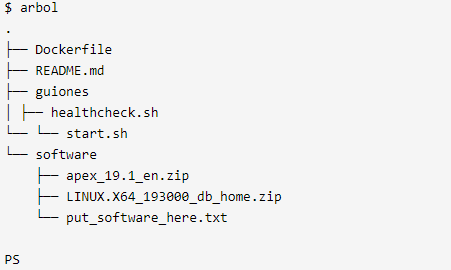
\includegraphics[width=8cm]{./Imagenes/100}
		\end{center}
		\end{figure}
	

\end{itemize}







